\section{Problem 4}
\label{part4}
\begin{verbatim}
Use MDS to create a JPEG of the blogs similar to slide 29.  
How many iterations were required??

\end{verbatim}

\subsection{Solution}
\begin{enumerate}
\item I was asked to use Multi-dimensional scaling to create a JPEG of the blogs similar to the figure in the lecture slides.
\item To do this I used ``clusters.py'' code from Programming Collective Intelligence text.
\item I have made modifications to ``cluster.py'' code to print the number of iterations. Number of Iterations taken are ``269''.
\item My code for generating the JPEG and printing the iterations can be found in listing\ref{lst:q4-1}.
\item JPEG image can be found in the following fig\ref{Sample4_t2} and sample list of the output can be found in this fig\ref{Sample4_t1}.
\end{enumerate}
\newpage

\subsection{Code Listing}
\subsubsection{Code Listing 1}

\lstinputlisting[language=Python,breaklines = true,frame=single,caption={Python code for creating a jpeg using mds}, label=lst:q4-1,captionpos=b,numbers=left,showspaces=false,showstringspaces=false,basicstyle=\footnotesize]{q4.py}
\newpage
\subsection{Outputs}
\subsubsection{Sample output file}
\begin{figure}[ht]    
    \begin{center}
        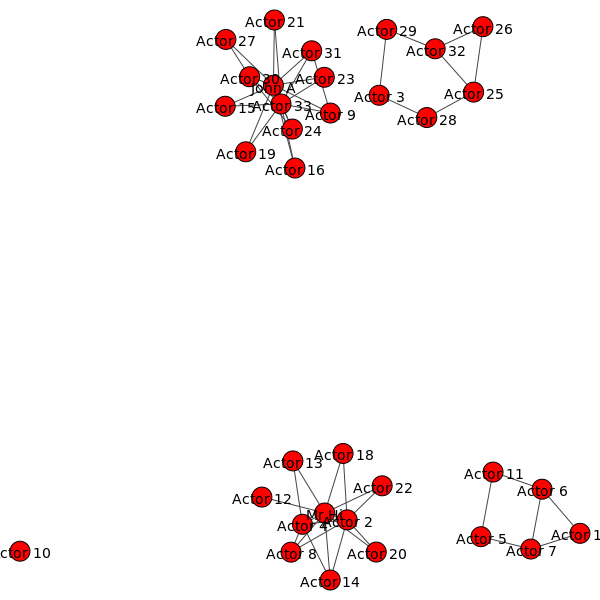
\includegraphics[scale=0.8]{output4.png}
        \caption{Sample list of iterations}
        \label{Sample4_t1}
    \end{center}
\end{figure}
\newpage
\subsubsection{jpeg file}
\begin{figure}[ht]    
    \begin{center}
        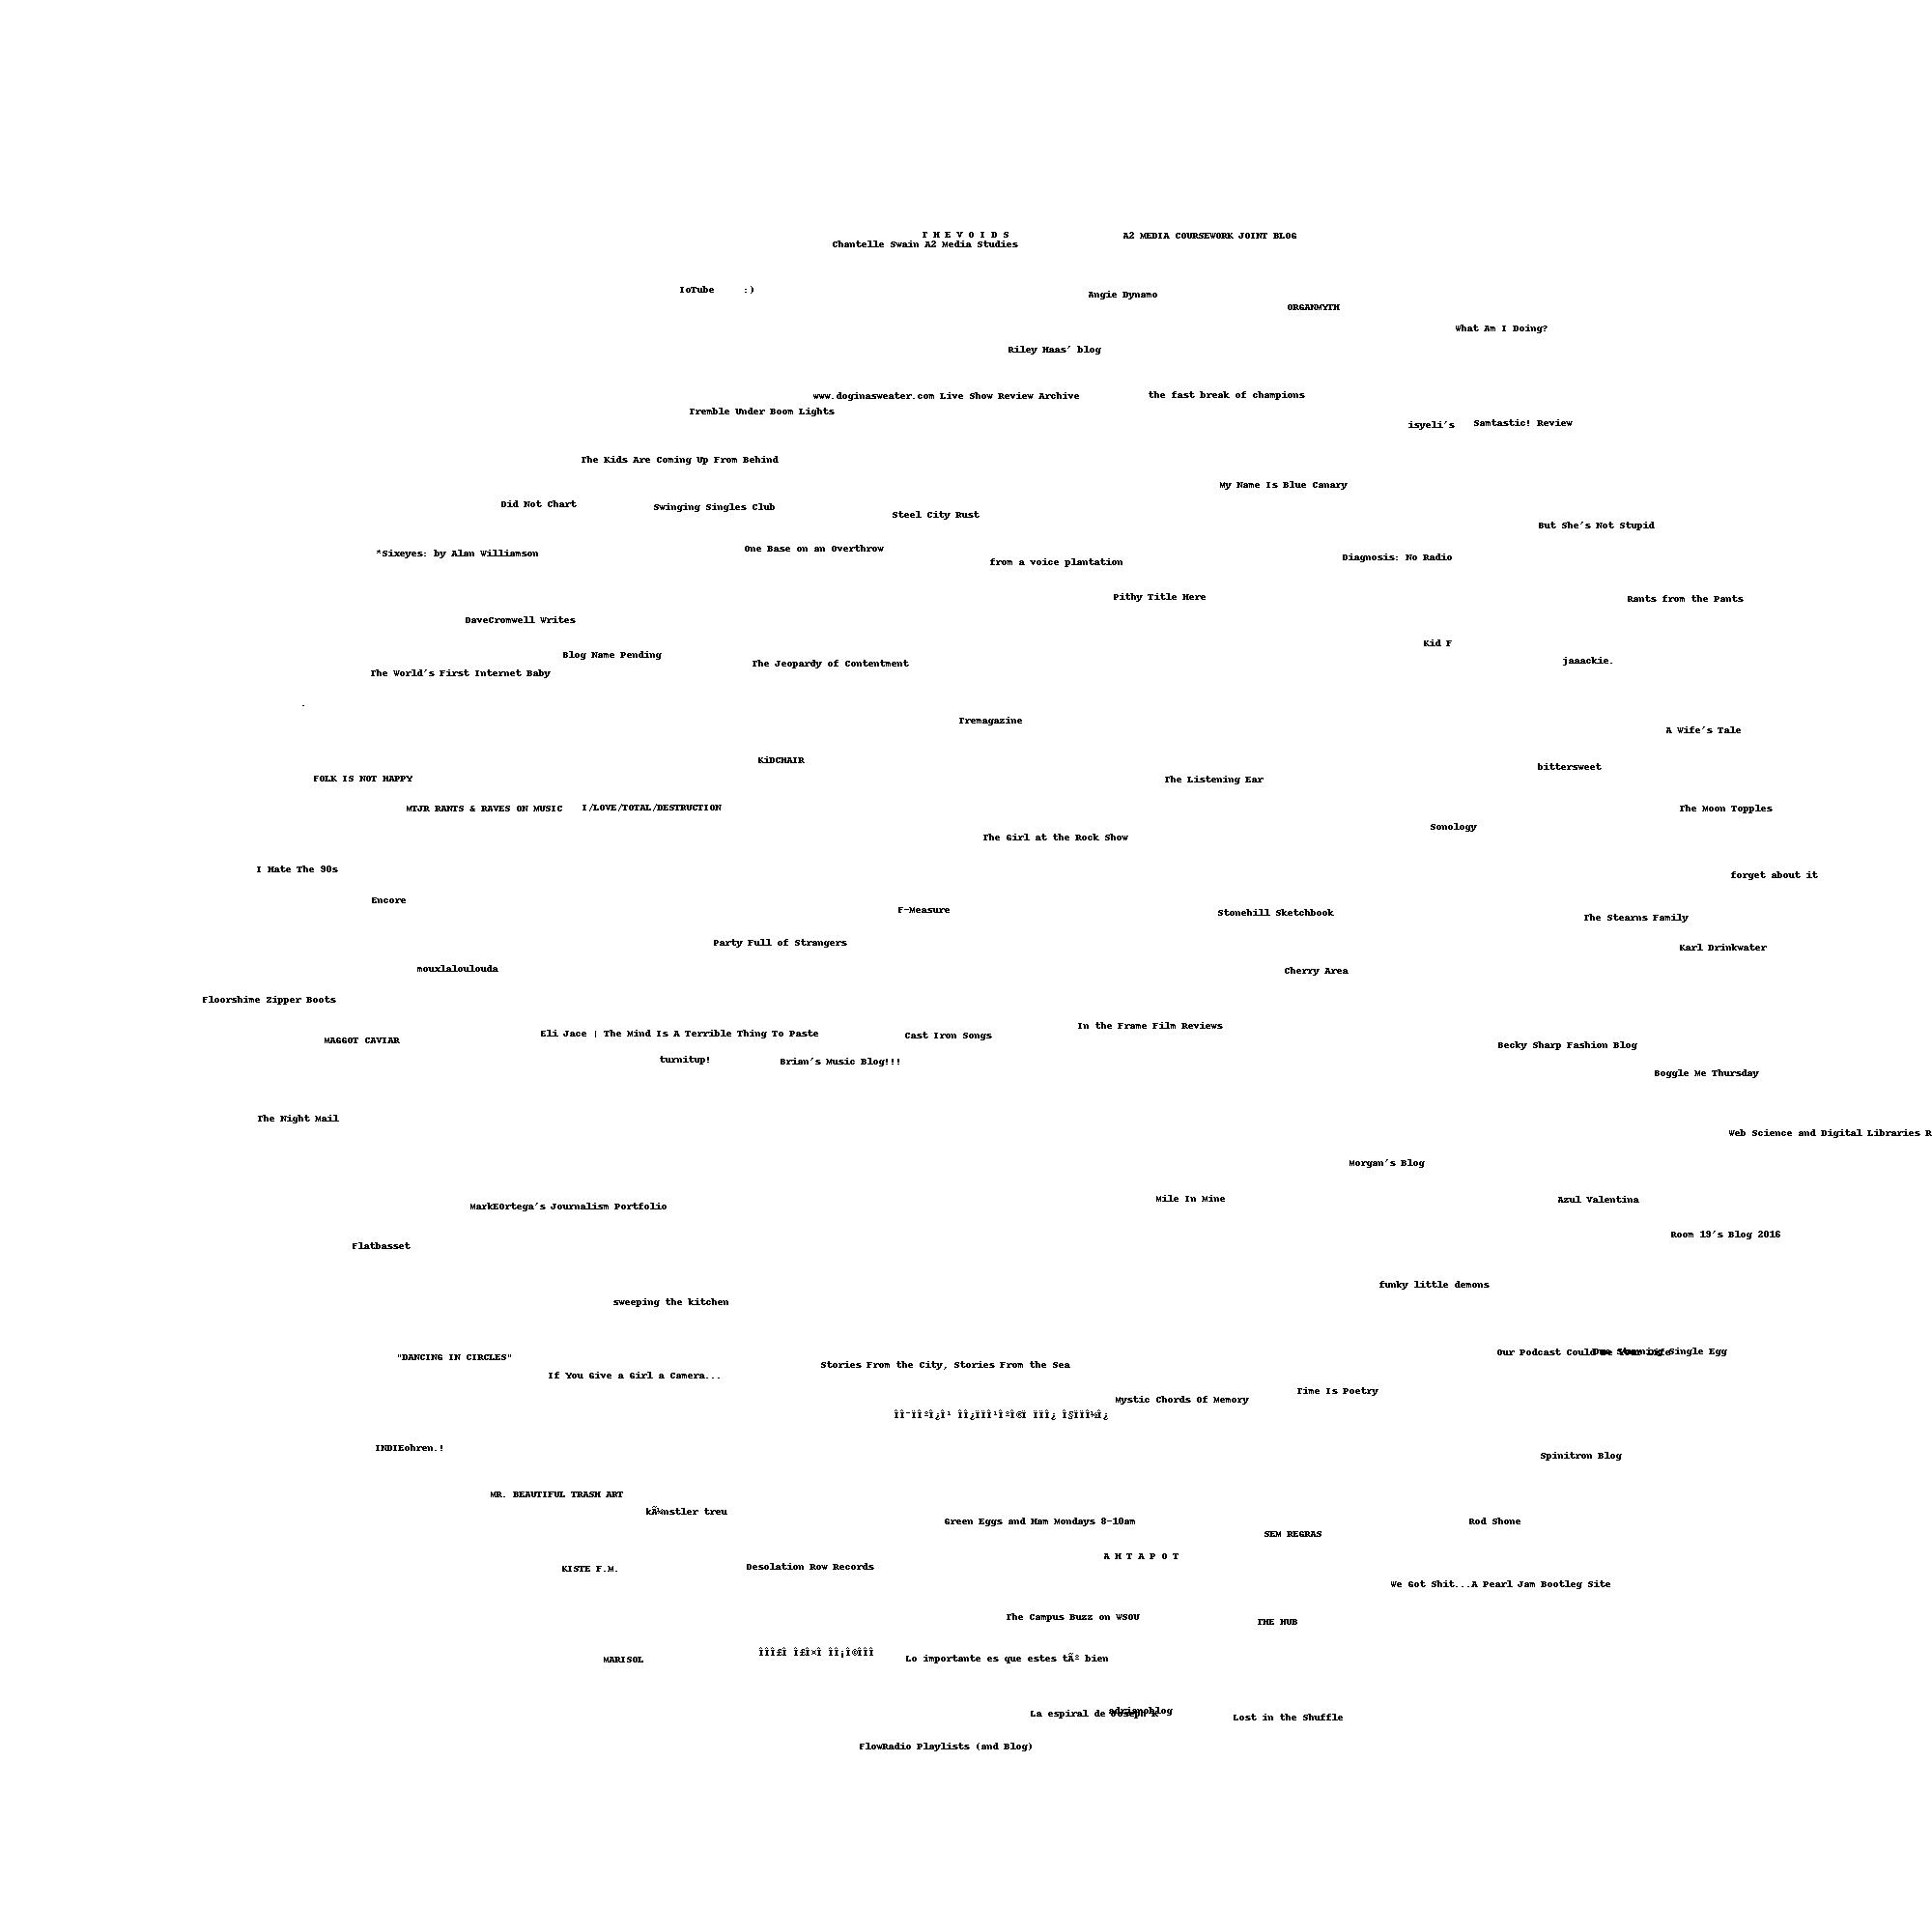
\includegraphics[scale=0.24]{blogs.jpg}
        \caption{Sample jpeg file representing blogs}
        \label{Sample4_t2}
    \end{center}
\end{figure}
\newpage

